\chapter{Grundlagen der Klassifikation}
\section{Gütemaße binärer Klassifikatoren}

Bei einer binären Klassifikation gibt es vier mögliche Klassifikationsergebnisse. Die beiden Klassen werden im allgemeinen als \emph{Positive} und \emph{Negative} beschrieben, was in diesem speziellen Fall \emph{Stimme} und \emph{Stille} entspricht. Eine Klassifikation, bei der ein tatsächliches Positive richtig als Positive vorhergesagt wird, spricht man von einem \emph{True Positive} [TP]. Wird hingegen ein tatsächliches Positive fälschlicherweise als Negative vorhergesagt, spricht man von einem \emph{False-Negative} [FN]. Das System wird entsprechend für die Klassifikation tatsächlicher Negatives angewandt und ergibt. \emph{True-Negatives} [TN] und \emph{False-Positives} [FP]. Die \emph{Confusion Matrix} in Abbildung \ref{img:Confusion-Matrix} gibt eine Übersicht über die vier möglichen Klassifikations-Ergebnisse.

\begin{figure}[h]
	\centering
	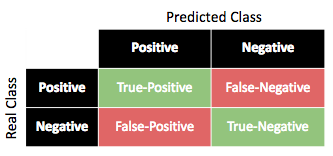
\includegraphics[width=0.3\textwidth]{bilder/Confusion-Matrix.png}
	\caption{Confusion-Matrix}
	\label{img:Confusion-Matrix}
\end{figure}

Die insgesamte Güte einer Klassifikation wird durch die \emph{Accuracy} nach Formel \ref{eq:accuracy} bestimmt. Eine Accuracy von 100\% bedeutet, dass \emph{alle} Instanzen richtig klassifiziert werden, eine Accuracy von 50\% bedeutet, dass die Hälfte aller instanzen richtig klassifiziert werden, was der Güte einer rein zufälligen Wahl entspricht.

\begin{equation}
\text{Accuracy} = \frac{TP+TN}{TP+TN+FN+FP}
\label{eq:accuracy}
\end{equation}

Die Accuracy beziffert die insgesamte Performance des Klassifikators, gibt jedoch keinen Aufschluss darüber, ob der Klassifikator eher eine Tendenz zur falschen Klassifizierung von Positives oder Negatives hat. Bei einer Datenbank mit der selben Anzahl an Positives und Negatives kann eine Accuracy von 50\% beispielsweise dadurch entstehen, dass \emph{alle} Instanzen als Positives markiert werden, also sowohl die Positives richtigerweise als Positives, aber die Negatives fälschlicherweise ebenfalls als Positives. Im Umgedrehten Fall ergibt die Klassifizierung aller Instanzen als Negatives ebenfalls eine Accuracy von 50\%. In einem dritten Fall irrt sich die Klassifikator gleich oft bei der Einordnung der Negatives und Positives.Die Maße \emph{Sensitivity} und \emph{Specificity} geben Aufschluss über die Güte der Klassifikation hinsichtlich der Positives und Negatives. Die \emph{Sensitivity}, auch bezeichnet als \emph{True-Positive-Rate}, bemisst den Anteil tatsächlicher Positives, die auch als solche erkannt wurden, nach Formel \ref{eq:sensitivity}. Eine Sensitivity von 100\% bedeutet, dass alle Positives durch den Klassifikator erkannt wurden. Die Erkennungsrate der Negatives hat keinen Einfluss auf die Sensitivity. Eine hohe Sensitivity lässt sich somit \glqq einfach\grqq{} erzielen, in dem man \emph{alle} Instanzen immer als Positives klassifiziert. Die Specificity nach Formel \ref{eq:specificity} bestimmt analog zur Sensitivity den Anteil der korrekt als Negatives bestimmten Instanzen. Ein Klassifikator, der alle Instanzen als Positives markiert, hat zwar eine Sensitivity von 100\%, aber eine Specificity von 0\%. Ergeben zwei verschiedene Klassifikationsmodelle sehr ähnliche Accuracies, hilft die Bestimmung der Sensitivity und Specificity bei der Auswahl des für den Anwendugnsfall Adequäteren Klassifikators. So ist beispielsweise bei der Bestimmung von schweren Krankheiten eventuell ein Klassifikator mit höherer Sensitivity wünschbar, um die Wahrscheinlichkeit zu minimieren, dass die entsprechende Krankheit nicht erkannt wird. \cite{sens-and_spec} \cite{accuracy}

\begin{equation}
\text{Sensitivity} = \frac{TP}{TP+FN}
\label{eq:sensitivity}
\end{equation}

\begin{equation}
\text{Specificity} = \frac{TN}{TN+FP}
\label{eq:specificity}
\end{equation}
\section{Klassifikationsalgorithmen}
\subsection{CARD}
\subsection{Andere}